\documentclass{standalone}
\usepackage{tikz-network}
\begin{document}
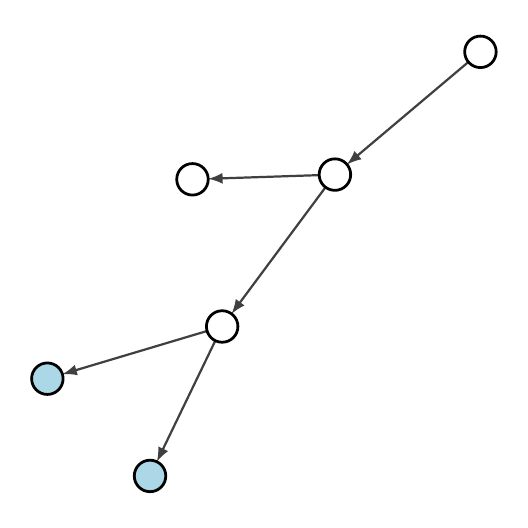
\begin{tikzpicture}
\clip (0,0) rectangle (6,6);
\Vertex[x=5.750,y=5.693,size=0.4,color=white,fontscale=0.857,shape=circle]{1}
\Vertex[x=3.902,y=4.134,size=0.4,color=white,fontscale=0.857,shape=circle]{2}
\Vertex[x=2.093,y=4.074,size=0.4,color=white,fontscale=0.857,shape=circle]{3}
\Vertex[x=2.470,y=2.205,size=0.4,color=white,fontscale=0.857,shape=circle]{4}
\Vertex[x=1.554,y=0.307,size=0.4,fontscale=0.857,shape=circle]{5}
\Vertex[x=0.250,y=1.542,size=0.4,fontscale=0.857,shape=circle]{6}
\Edge[,lw=0.8,bend=0,Direct](1)(2)
\Edge[,lw=0.8,bend=0,Direct](2)(3)
\Edge[,lw=0.8,bend=0,Direct](2)(4)
\Edge[,lw=0.8,bend=0,Direct](4)(5)
\Edge[,lw=0.8,bend=0,Direct](4)(6)
\end{tikzpicture}
\end{document}